
\documentclass[11pt]{article}

\usepackage{amsmath}
\usepackage{amsfonts}
\usepackage{indentfirst}

\DeclareMathOperator{\var}{var}
\newcommand{\Prmu}{\Pr\nolimits_\mu}
\newcommand{\Prsub}[1]{\Pr\nolimits_{#1}}

\newcommand{\real}{\mathbb{R}}

\newcommand{\set}[1]{\{\, #1 \,\}}

% \VignetteIndexEntry{Design Document for Truncated Distributions}

\usepackage{/APPS/64//lib64/R/share/texmf/Sweave}
\begin{document}

\title{Lower-Truncated Poisson and Negative Binomial Distributions}
\author{Charles J. Geyer}
\maketitle


\section{Introduction}

This document works through the details of the $k$-truncated Poisson
distribution and the $k$-truncated negative binomial distribution,
which are the distributions of $Y$ conditioned on $Y > k$, where $k$
is a nonnegative integer and $Y$ has a Poisson or negative binomial
distribution.  It is a design document.  There is no reason for ordinary
users to read it (except perhaps curiosity).  It written for developers.

The negative binomial distribution with \emph{shape parameter $\alpha$}
and \emph{mean parameter $\mu$} has probability mass function (PMF)
$$
   f_{\alpha, \mu}(y)
   =
   \frac{\Gamma(y + \alpha)}{\Gamma(\alpha) y !} p^\alpha (1 - p)^y,
   \qquad y = 0, 1, 2, \ldots,
$$
where
$$
   p = \frac{\alpha}{\alpha + \mu}.
$$
If one takes the limit as $\alpha \to \infty$ holding $\mu$ fixed,
one obtains
$$
   f_{\infty, \mu}(y)
   =
   \frac{\mu^y}{y !} e^{- \mu}
   \qquad y = 0, 1, 2, \ldots,
$$
which defines the PMF of the Poisson distribution
with \emph{mean parameter $\mu$}
(we do not prove this, because we do not use this limit in any way
and only mention it to explain why we use the $\infty$ subscript to
denote the Poisson PMF).

The PMF of the $k$-truncated distribution corresponding to the (untruncated)
distribution with parameters $\alpha$ and $\mu$ has PMF defined by
\begin{equation} \label{eq:pmf-trunc-one}
   f_{k, \alpha, \mu}(x)
   =
   \frac{f_{\alpha, \mu}(x)}{\Prsub{\alpha, \mu}\{Y > k\}},
   \qquad x = k + 1, k + 2, \ldots,
\end{equation}
where $\Prsub{\alpha, \mu}$ indicates probability calculated with
respect to the untruncated distribution.

\section{Exponential Family Properties}

\subsection{Untruncated Families}

\subsubsection{Probability Mass Function}

The negative binomial distribution and Poisson are both exponential families.
Their densities have the form
\begin{equation} \label{eq:pmf-exp-fam}
   f_{\alpha, \mu} = \frac{1}{c_\alpha(\theta)} e^{y \theta} m_\alpha(y),
   \qquad y = 0, 1, 2, \ldots.
\end{equation}
The function
$c_\alpha$ is called the \emph{Laplace transform} of the family.
The function $m_\alpha$ is called the \emph{base measure} of the family.
The parameter $\theta$ is called the \emph{canonical parameter} of the
family.  We have a different exponential family for each $\alpha$.
If we were to consider this a two-parameter family with parameters
$\alpha$ and $\theta$, then it would not have exponential family form.

In order that probabilities sum to one, we must have
\begin{equation} \label{eq:lap-tr}
   c_\alpha(\theta) = \sum_{y = 0}^\infty e^{y \theta} m_\alpha(y),
\end{equation}
so the choice of base measure determines the family.
We consider \eqref{eq:lap-tr} to define a function on all of $\real$
(the real number system), taking the value $+ \infty$ when the sum in
\eqref{eq:lap-tr} does not converge (which makes sense because all terms
in the sum are nonnegative).  This allows us to define the
\emph{canonical parameter space} of the family as the set
$$
   \Theta_\alpha = \set{ \theta \in \real : c_\alpha(\theta) < \infty }.
$$
Then \eqref{eq:pmf-exp-fam} defines a PMF for all $\theta \in \Theta_\alpha$.

\paragraph{Poisson}

To get the Poisson distribution, we define the base measure by
$$
   m_\infty(y) = \frac{1}{y !}
$$
Then we must have
$$
   e^{y \theta} = \mu^y
$$
from which we see that the transformations between the original parameter
$\mu$ and the canonical parameter $\theta$ are $\mu = \exp(\theta)$ and
$\theta = \log(\mu)$.

The Laplace transform is then seen to be
$$
   c_\infty(\theta) = e^\mu = e^{e^\theta} = \exp(\exp(\theta))
$$
and the canonical parameter space $\Theta_\infty$ is the whole
real line.

\paragraph{Negative Binomial}

To get the negative binomial distribution, we define the base measure by
$$
   m_\alpha(y) = \frac{\Gamma(y + \alpha)}{\Gamma(\alpha) y !}
$$

Then we must have
$$
   e^{y \theta} = (1 - p)^y = \left( \frac{\mu}{\mu + \alpha} \right)^y
$$
from which we see that the transformations between
the \emph{success probability parameter $p$} and the
canonical parameter $\theta$ are $\theta = \log(1 - p)$ and $p = 1 - e^\theta$
and that the transformations between the mean parameter $\mu$ and
the canonical parameter $\theta$ are $\theta = \log(\mu) - \log(\mu + \alpha)$
and
\begin{equation} \label{eq:theta-to-mu-neg-bin}
   \mu
   =
   \alpha \cdot \frac{e^\theta}{1 - e^\theta}
   =
   \alpha \cdot \frac{1 - p}{p}
\end{equation}

The Laplace transform is then seen to be
\begin{equation} \label{eq:lap-tr-neg-bin}
   c_\alpha(\theta) = p^{- \alpha}
   = \left(1 + \frac{\mu}{\alpha} \right)^\alpha
   = \left(1 + \frac{1}{e^{- \theta} - 1} \right)^\alpha
\end{equation}
Since all the $y$ in \eqref{eq:lap-tr} are positive, $c_\alpha$ is
nondecreasing.
To have $0 < p < 1$, we must also have $\theta < 0$.  We see
that \eqref{eq:lap-tr-neg-bin} makes sense for such $\theta$ and
that $c_\alpha(\theta) \to + \infty$ as $\theta \uparrow 0$.
Hence
$$
   \Theta_\alpha = \set{ \theta \in \real : \theta < 0 }.
$$

\subsubsection{Cumulant Function and its Derivatives}

The log Laplace transform is called the \emph{cumulant function} because
its derivatives are cumulants of the distributions in the family.
We write
$$
   \psi_\alpha(\theta) = \log c_\alpha(\theta)
$$
to define the cumulant function.

Then from standard exponential family theory
\begin{align*}
   \psi_\alpha'(\theta) & = E_{\alpha, \theta}(Y)
   \\
   \psi_\alpha''(\theta) & = \var_{\alpha, \theta}(Y)
\end{align*}
One can directly verify this in any particular case by evaluating the
derivatives.

\paragraph{Poisson}

\begin{subequations}
\begin{align}
   \psi_\infty(\theta) & = e^\theta
   \label{eq:cum-fun-pois}
   \\
   \psi_\infty'(\theta) & = e^\theta
   \\
   \psi_\infty''(\theta) & = e^\theta
   \label{eq:cum-fun-pp-pois}
\end{align}
\end{subequations}

\paragraph{Negative Binomial}

\begin{subequations}
\begin{align}
   \psi_\alpha(\theta) & = 
   \alpha \log \left(1 + \frac{1}{e^{- \theta} - 1} \right)
   \label{eq:cum-fun-neg-bin}
   \\
   \psi_\alpha'(\theta) & = \alpha \cdot \frac{e^\theta}{1 - e^\theta}
   \\
   \psi_\alpha''(\theta) & = \alpha \cdot \frac{e^\theta}{(1 - e^\theta)^2}
   \label{eq:cum-fun-pp-neg-bin}
\end{align}
\end{subequations}
Written in terms of the more familiar success probability parameter
we have
\begin{align*}
   \psi_\alpha'(\theta) & = \alpha \cdot \frac{1 - p}{p}
   \\
   \psi_\alpha''(\theta) & = \alpha \cdot \frac{1 - p}{p^2}
\end{align*}
giving the usual formulas for the mean and variance of a negative
binomial random variable.

\subsection{Truncated Families}

The relationship between the PMF of truncated and untruncated families
has already been given in \eqref{eq:pmf-trunc-one}.
Since $\Prsub{\alpha, \mu}\{Y > k\}$ does not involve the data $x$,
we see we again have an exponential family with the same canonical parameter
and same canonical parameter space but with Laplace transform
$$
   c_{k, \alpha}(\theta) = c_\alpha(\theta) \Prsub{\alpha, \mu}\{Y > k\}
$$
and hence
\begin{equation*}
   \psi_{k, \alpha}(\theta)
   =
   \psi_\alpha(\theta)
   +
   \log \Prsub{\alpha, \mu}\{Y > k\}
\end{equation*}
where $\mu$ is given as a function of $\theta$ by
$\mu = \exp(\theta)$ for the Poisson and
\eqref{eq:theta-to-mu-neg-bin} for the negative binomial.
Hence we can also write this
\begin{equation} \label{eq:cum-funk}
   \psi_{k, \alpha}(\theta)
   =
   \psi_\alpha(\theta)
   +
   \log \Prsub{\alpha, \theta}\{Y > k\}
\end{equation}

The mean and variance of $X$ are again given by the first and second
derivatives of the cumulant function \eqref{eq:cum-funk}
\begin{subequations}
\begin{align}
   \psi_{k, \alpha}'(\theta)
   & =
   E_{k, \alpha, \theta}\{ X \}
   =
   E_{\alpha, \theta}\{ Y \mid Y > k \}
   \label{eq:tau-funk}
   \\
   \psi_{k, \alpha}''(\theta)
   & =
   \var_{k, \alpha, \theta}\{ X \}
   =
   \var_{\alpha, \theta}\{ Y \mid Y > k \}
   \label{eq:tau-prime-funk}
\end{align}
\end{subequations}
These identities must hold by exponential family theory.
Of course, they can also be verified directly by evaluating the
derivatives seeing that they do indeed give the appropriate expectation.

Note that although we still use $\mu$ as a parameter, it is no longer
the mean of the $k$-truncated variable $X$ (it is the mean of the
corresponding untruncated variable $Y$).  The mean of $X$ is yet another
parameter
\begin{equation} \label{eq:mvp}
   \tau = \psi_{k, \alpha}'(\theta)
\end{equation}
which is called the \emph{mean value parameter} of the family.
The fact that
$$
   \frac{d \tau}{d \theta} = \var_{k, \alpha, \theta}(X)
$$
is necessarily positive (because it is a variance) means
the map $\theta \mapsto \tau$ is one-to-one, an invertible
change-of-parameter.  We will make no use of this fact.
The only point of this paragraph is to stress that
the mean of $X$ is not $\mu$; the mean of $X$ is $\tau$.

\section{Computing}

As always, we wish to compute things, in this case the cumulant function
and its first two derivatives, without overflow or cancellation error.
Problems arise when $\mu$ is nearly zero or when $\mu$ is very large.

\subsection{Cumulant Function}

We consider \eqref{eq:cum-funk} fairly behaved computationally.
The computation of $\log \Prsub{\alpha, \theta}\{Y > k\}$ can be left
to the relevant R function (\verb@ppois@ or \verb@pnbinom@) using
the \verb@lower.tail = FALSE@ and \verb@log.p = TRUE@ optional arguments
to avoid cancellation error and overflow.
% Actually, this optimism about R coding seems justified only for the
% \verb@ppois@ function.  Negative binomial probabilities should be
% coded
% \begin{verbatim}
%     log1p(- pnbinom(k, size = alpha, mu = mu))
% \end{verbatim}
% to avoid underflow for large \verb@mu@.

Any of the cumulant functions we are discussing are
continuous, because differentiable, and strictly increasing,
because their derivatives are the mean value parameters, which are strictly
positive.  It can be checked directly from \eqref{eq:cum-fun-pois}
and \eqref{eq:cum-fun-neg-bin} that
\begin{align*}
   \psi_\alpha(\theta) \to 0, & \qquad \text{as $\theta \to - \infty$}
   \\
   \psi_\alpha(\theta) \to + \infty,
   & \qquad \text{as $\theta \to \sup \Theta_\alpha$}
\end{align*}
where, of course, $\sup \Theta_\alpha$ is zero for the negative binomial
and $+ \infty$ for the Poisson.
It can also be checked directly that
\begin{align*}
   \Prsub{\alpha, \theta}\{Y > k\} \to 0,
   & \qquad \text{as $\theta \to - \infty$}
   \\
   \Prsub{\alpha, \theta}\{Y > k\} \to 1,
   & \qquad \text{as $\theta \to \sup \Theta_\alpha$}
\end{align*}
hence
\begin{align*}
   \log \Prsub{\alpha, \theta}\{Y > k\} \to - \infty,
   & \qquad \text{as $\theta \to - \infty$}
   \\
   \log \Prsub{\alpha, \theta}\{Y > k\} \to 0,
   & \qquad \text{as $\theta \to \sup \Theta_\alpha$}
\end{align*}

Thus $\psi_{k, \alpha}$, which is also continuous and strictly increasing
(because its derivative is strictly positive), goes from $- \infty$
to $+ \infty$
as $\theta$ goes from the lower end of $\Theta_\alpha$ to the upper end.

Since the addition in the computation of \eqref{eq:cum-funk} involves
terms of opposite sign, $\psi_{k, \alpha}(\theta)$ positive and
$\log \Prsub{\alpha, \theta}\{Y > k\}$ negative, cancellation error may occur.
Also overflow to \verb@-Inf@ or \verb@Inf@
(if the machine arithmetic is IEEE, as is true with most machines nowadays)
may occur when $\theta$ is near an endpoint of $\Theta_\alpha$,

What cannot happen is that we get \verb@-Inf + Inf = NaN@ (in IEEE arithmetic)
because when the first term is large, the second is near zero, and vice versa.
Thus we regard whatever cancellation error occurs as not a problem.
There seems to be nothing that can be done about it if we use the
floating-point arithmetic native to the machine.

\subsection{First Derivative of Cumulant Function}

In evaluating derivatives of \eqref{eq:cum-funk}, we have no
problem evaluating derivatives of $\psi_\alpha(\theta)$.
The only problematic part is derivatives of
$\log \Prsub{\alpha, \theta}\{Y > k\}$.
Since we have no formulas for that, we proceed differently.

From \eqref{eq:tau-funk} we have
\begin{align*}
   \psi_{k, \alpha}'(\theta)
   & =
   E_{\alpha, \theta}\{ Y \mid Y > k \}
   \\
   & =
   \frac{E_{\alpha, \theta}\{ Y I(Y > k) \}}
   {\Prsub{\alpha, \theta}\{Y > k\}}
\end{align*}
where $Y$ denotes a random variable having the corresponding
untruncated distribution, and $I(Y > k)$ is one if $Y > k$ and zero otherwise.
There being no functions that evaluate expectations with respect
to Poisson and negative binomial distributions, we need to rewrite
this in terms of probabilities using special properties of each distribution.

\subsubsection{Poisson}

\begin{equation} \label{eq:trick-pois}
\begin{split}
   E_{\infty, \theta}\{ Y I(Y > k) \}
   & =
   \sum_{y = k + 1}^\infty \frac{\mu^y}{(y - 1) !} e^{- \mu}
   \\
   & =
   \mu \Prsub{\infty, \theta}\{Y \ge k\}
\end{split}
\end{equation}
Hence
\begin{align*}
   E_{\infty, \theta}\{ Y \mid Y > k \}
   & =
   \frac{\mu \Prsub{\infty, \theta}\{Y \ge k\}}
   {\Prsub{\infty, \theta}\{Y > k\}}
   \\
   & =
   \mu + \frac{\mu \Prsub{\infty, \theta}\{Y = k\}}
   {\Prsub{\infty, \theta}\{Y > k\}}
   \\
   & =
   \mu +
   \frac{\mu^{k + 1} e^{- \mu} / k !}
   {\mu^{k + 1} e^{- \mu} / (k + 1) ! + \Prsub{\infty, \theta}\{Y > k + 1 \}}
   \\
   & =
   \mu +
   \frac{k + 1}
   {1 + \frac{\Prsub{\infty, \theta}\{Y > k + 1 \}}
   {\Prsub{\infty, \theta}\{Y = k + 1 \}}}
\end{align*}
To simplify notation we give the fraction in the denominator a name
\begin{equation} \label{eq:beta}
   \beta = \frac{\Prsub{\alpha, \theta}\{Y > k + 1 \}}
   {\Prsub{\alpha, \theta}\{Y = k + 1 \}}
\end{equation}
(We use subscript $\alpha$ because we will use the same definition of
$\beta$ for both cases.  The Poisson case has $\alpha = \infty$.)
Then
\begin{equation} \label{eq:tau-comp-pois}
   \psi_{k, \infty}'(\theta) = \mu + \frac{k + 1}{1 + \beta}
\end{equation}
We are pleased with this formula, which took a bit of formula bashing
to find, since it behaves very well computationally.

Since both terms in \eqref{eq:tau-comp-pois} are positive, we never have
cancellation error.  When $\mu$ is near zero, we have $\beta$ near zero,
and \eqref{eq:tau-comp-pois} calculates a result near $k + 1$ accurately.
When $\mu$ is large, we have $\beta$ also large,
and \eqref{eq:tau-comp-pois} calculates a result near $\mu$ accurately.
The result may overflow (to \verb@Inf@ in IEEE arithmetic), but only
when $\mu$ itself is near overflow.

\subsubsection{Negative Binomial}

\begin{align*}
   E_{\alpha, \theta} \{ Y I(Y > k) \}
   & =
   \sum_{y = k + 1}^\infty
   y \frac{\Gamma(y + \alpha)}{\Gamma(\alpha) y!} p^\alpha (1 - p)^y
   \\
   & =
   (1 - p)
   \sum_{y = k + 1}^\infty
   (y - 1 + \alpha)
   \frac{\Gamma(y - 1 + \alpha)}{\Gamma(\alpha) (y - 1)!}
   p^\alpha (1 - p)^{y - 1}
   \\
   & =
   (1 - p)
   E_{\alpha, \theta} \{ (Y + \alpha) I(Y \ge k) \}
   \\
   & =
   (1 - p)
   E_{\alpha, \theta} \{ Y I(Y \ge k) \}
   +
   \alpha (1 - p) \Prsub{\alpha, \theta} \{ Y \ge k \}
   \\
   & =
   (1 - p)
   E_{\alpha, \theta} \{ Y I(Y > k) \}
   +
   k (1 - p) \Prsub{\alpha, \theta} \{ Y = k \}
   \\
   & \qquad
   +
   \alpha (1 - p) \Prsub{\alpha, \theta} \{ Y \ge k \}
\end{align*}
Moving the term containing the expectation (rather than probability)
from the right hand side to the left, we obtain
\begin{equation} \label{eq:fred}
\begin{split}
   p E_{\alpha, \theta} \{ Y I(Y > k) \}
   & =
   k (1 - p) \Prsub{\alpha, \theta} \{ Y = k \}
   +
   \alpha (1 - p) \Prsub{\alpha, \theta} \{ Y \ge k \}
   \\
   & =
   (k + \alpha) (1 - p) \Prsub{\alpha, \theta} \{ Y = k \}
   +
   \alpha (1 - p) \Prsub{\alpha, \theta} \{ Y > k \}
\end{split}
\end{equation}
and have expressed this expectation in terms of probability functions
(which are implemented in R).

Hence
\begin{equation} \label{eq:tau-comp-one}
\begin{split}
   E_{\alpha, \theta}\{ Y \mid Y > k \}
   & =
   \frac{\alpha (1 - p)}{p}
   +
   \frac{(k + \alpha) (1 - p) \Prsub{\alpha, \theta} \{ Y = k \}}
   {p \Prsub{\alpha, \theta} \{ Y > k \}}
   \\
   & =
   \mu +
   \frac{(k + \alpha) (1 - p) \Prsub{\alpha, \theta} \{ Y = k \}}
   {p \Prsub{\alpha, \theta} \{ Y > k \}}
\end{split}
\end{equation}
We work on
\begin{align*}
   (1 - p) (k + \alpha) \Prsub{\alpha, \theta} \{Y = k\}
   & =
   (1 - p) (k + \alpha)
   \frac{\Gamma(k + \alpha)}{\Gamma(\alpha) k !} p^\alpha (1 - p)^k
   \\
   & =
   \frac{\Gamma(k + 1 + \alpha)}{\Gamma(\alpha) k !} p^\alpha (1 - p)^{k + 1}
   \\
   & =
   (k + 1) \frac{\Gamma(k + 1 + \alpha)}{\Gamma(\alpha) (k + 1) !}
   p^\alpha (1 - p)^{k + 1}
   \\
   & =
   (k + 1) \Prsub{\alpha, \theta} \{ Y = k + 1 \}
\end{align*}
Hence
\begin{align*}
   E_{\alpha, \theta}\{ Y \mid Y > k \}
   & =
   \mu +
   \frac{(k + 1) \Prsub{\alpha, \theta} \{ Y = k + 1 \}}
   {p \Prsub{\alpha, \theta} \{ Y > k \}}
   \\
   & =
   \mu +
   \frac{(k + 1)}
   {p + p \frac{\Prsub{\alpha, \theta} \{ Y > k + 1 \}}
   {\Prsub{\alpha, \theta} \{ Y = k + 1 \}}}
\end{align*}
Defining $\beta$ by \eqref{eq:beta} as in the Poisson case, we get
\begin{equation} \label{eq:tau-comp-neg-bin}
   \psi_{k, \alpha}'(\theta) = \mu + \frac{k + 1}{p (1 + \beta)}
\end{equation}
as our simple computational formula for the mean value parameter
in the negative binomial case.
Formula \eqref{eq:tau-comp-neg-bin} is not as well behaved as
its Poisson analogue \eqref{eq:tau-comp-pois}, but only in that we
can have $p$ underflow to zero and $\Prsub{\alpha, \theta} \{ Y = k + 1 \}$
also underflow to zero, giving a possible \verb@NaN@ result
for $p (1 + \beta)$.  However, when $p$ underflows to zero,
$\mu$ evaluates to \verb@Inf@, and hence \eqref{eq:tau-comp-neg-bin},
being the sum of positive terms should evaluate to \verb@Inf@ as well.
Thus, if we simply return \verb@Inf@ when computing \eqref{eq:tau-comp-neg-bin}
and \verb@p == 0.0@, we avoid \verb@NaN@ and produce a correct result.
We may produce \verb@Inf@, but consider that not a problem.

In testing (Section~\ref{sec:check} below) we discovered another
issue.  The R functions \verb@pnbinom@ and \verb@dnbinom@ just punt
on very small $\mu$ and so $\beta$ can be calculated as \verb@0.0 / 0.0 = NaN@
when $\mu$ is very near zero (and $\theta$ very large negative).
What should we get in this case?  From \eqref{eq:beta}
\begin{align*}
   \beta
   & =
   \frac{\Prsub{\alpha, \theta}\{Y > k + 1 \}}
   {\Prsub{\alpha, \theta}\{Y = k + 1 \}}
   \\
   & =
   \frac{
   \sum_{y = k + 2}^\infty
   \frac{\Gamma(y + \alpha)}{\Gamma(\alpha) y !} p^\alpha (1 - p)^y}
   {\frac{\Gamma(k + 1 + \alpha)}{\Gamma(\alpha) (k + 1) !}
   p^\alpha (1 - p)^{k + 1}}
   \\
   & =
   \frac{(k + 1) !}{\Gamma(k + 1 + \alpha)}
   \sum_{y = k + 2}^\infty
   \frac{\Gamma(y + \alpha)}{y !} (1 - p)^{y - (k + 1)}
\end{align*}
Now $1 - p \to 0$ as $\mu \to 0$ and the sum in the last expression
converges to zero (by dominated convergence).
Thus we should replace \verb@NaN@ calculated for $\beta$ when $\mu$ is
near zero by zero.

\subsection{Second Derivative of Cumulant Function}

We obtain a formula for the second derivative of $\psi_{k, \alpha}$
by differentiating our computationally stable formulas
\eqref{eq:tau-comp-pois} and \eqref{eq:tau-comp-neg-bin} and using
$$
   \frac{\partial \mu}{\partial \theta} = \psi_\alpha''(\theta)
$$
for which we already have the formulas \eqref{eq:cum-fun-pp-pois}
and \eqref{eq:cum-fun-pp-neg-bin} so we only need formulas for the derivatives
of the second terms on the right hand sides
of \eqref{eq:tau-comp-pois} and \eqref{eq:tau-comp-neg-bin}.

\subsubsection{Poisson}

\begin{align*}
   \frac{\partial}{\partial \theta}
   \left(
   \frac{k + 1}{1 + \beta}
   \right)
   & =
   -
   \frac{k + 1}{(1 + \beta)^2}
   \cdot
   \frac{\partial \beta}{\partial \theta}
\end{align*}
and
\begin{align*}
   \frac{\partial \beta}{\partial \theta}
   & =
   \frac{\partial}{\partial \theta}
   \left(
   \frac{\Prsub{\infty, \theta}\{Y > k + 1 \}}
   {\Prsub{\infty, \theta}\{Y = k + 1 \}}
   \right)
   \\
   & =
   \frac{\partial}{\partial \theta}
   \sum_{y = k + 2}^\infty \frac{e^{[y - (k + 1)] \theta} (k + 1) !}{y !}
   \\
   & =
   \sum_{y = k + 2}^\infty [y - (k + 1)]
   \frac{e^{[y - (k + 1)] \theta} (k + 1) !}{y !}
   \\
   & =
   \frac{E_{\infty, \theta} \{ [Y - (k + 1)] I(Y > k + 1) \}}
   {\Prsub{\infty, \theta}\{Y = k + 1 \}}
   \\
   & =
   \frac{E_{\infty, \theta} \{ Y I(Y > k + 1) \} -
   (k + 1) \Prsub{\infty, \theta} \{ Y > k + 1 \} }
   {\Prsub{\infty, \theta}\{Y = k + 1 \}}
   \\
   & =
   \frac{ \mu \Prsub{\infty, \theta}\{Y \ge k + 1 \} -
   (k + 1) \Prsub{\infty, \theta} \{ Y > k + 1 \} }
   {\Prsub{\infty, \theta}\{Y = k + 1 \}}
   \\
\intertext{the preceding step resulting from plugging in \eqref{eq:trick-pois}}
   & =
   \frac{ \mu \Prsub{\infty, \theta}\{Y = k + 1 \} +
   [\mu - (k + 1)] \Prsub{\infty, \theta} \{ Y > k + 1 \} }
   {\Prsub{\infty, \theta}\{Y = k + 1 \}}
   \\
   & =
   \mu \left( 1 + \beta - \frac{k + 1}{\mu} \beta \right)
\end{align*}
Putting this all together we get
\begin{equation} \label{eq:psi-double-prime-comp-pois}
   \psi_{k, \infty}''(\theta)
   =
   \mu
   \left[ 1 - \frac{k + 1}{1 + \beta}
   \left( 1 - \frac{k + 1}{\mu} \cdot \frac{\beta}{1 + \beta} \right) \right]
\end{equation}
The only particular care required in
evaluating \eqref{eq:psi-double-prime-comp-pois} is to evaluate
$\beta / (1 + \beta)$ as written when $\beta$ is small but
as $1 / (1 / \beta + 1)$ when $\beta$ is large.

\subsubsection{Negative Binomial}

\begin{align*}
   \frac{\partial}{\partial \theta}
   \left(
   \frac{k + 1}{p (1 + \beta)}
   \right)
   & =
   -
   \frac{k + 1}{(1 + \beta)^2}
   \left(
   \frac{\partial p}{\partial \theta} (1 + \beta)
   +
   p \frac{\partial \beta}{\partial \theta}
   \right)
\end{align*}
and
\begin{align*}
   \frac{\partial p}{\partial \theta}
   & =
   \frac{\partial}{\partial \theta}
   (1 - e^\theta)
   \\
   & =
   - e^\theta
   \\
   & =
   - (1 - p)
\end{align*}
and
\begin{align*}
   \frac{\partial \beta}{\partial \theta}
   & =
   \frac{\partial}{\partial \theta}
   \sum_{y = k + 2}^\infty
   \frac{
   \frac{\Gamma(y + \alpha)}{\Gamma(\alpha) y!} p^\alpha (1 - p)^y
   }{
   \frac{\Gamma(k + 1 + \alpha)}{\Gamma(\alpha) (k + 1)!}
   p^\alpha (1 - p)^{k + 1}
   }
   \\
   & =
   \frac{\partial}{\partial \theta}
   \sum_{y = k + 2}^\infty
   \frac{\Gamma(y + \alpha)}{\Gamma(k + 1 + \alpha)}
   \cdot
   \frac{(k + 1)!}{y!}
   \cdot
   e^{[y - (k + 1)] \theta}
   \\
   & =
   \frac{\partial}{\partial \theta}
   \sum_{y = k + 2}^\infty
   \frac{\Gamma(y + \alpha)}{\Gamma(k + 1 + \alpha)}
   \cdot
   \frac{(k + 1)!}{y!}
   \cdot
   (1 - p)^{y - (k + 1)}
   \cdot
   [y - (k + 1)]
   \\
   & =
   \frac{E_{\alpha, \theta}\{[Y - (k + 1)] I(Y > k + 1)\}}
   {\Prsub{\alpha, \theta} \{Y = k + 1\}}
\end{align*}
So
\begin{align*}
   p \frac{\partial \beta}{\partial \theta}
   & =
   \frac{p E_{\alpha, \theta}\{[Y - (k + 1)] I(Y > k + 1)\}}
   {\Prsub{\alpha, \theta} \{Y = k + 1\}}
   \\
   & =
   \frac{p E_{\alpha, \theta}\{Y I(Y > k + 1)\}
   - p (k + 1) \Prsub{\alpha, \theta} \{Y > k + 1\}}
   {\Prsub{\alpha, \theta} \{Y = k + 1\}}
   \\
\intertext{which using \eqref{eq:fred} becomes}
   & =
   \frac{1}{\Prsub{\alpha, \theta} \{Y = k + 1\}} \bigl[
   (k + 1 + \alpha) (1 - p) \Prsub{\alpha, \theta}  \{ Y = k + 1 \}
   \\
   & \qquad
   +
   \alpha (1 - p) \Prsub{\alpha, \theta}  \{ Y > k + 1 \}
   - p (k + 1) \Prsub{\alpha, \theta} \{Y > k + 1\} \bigr]
   \\
   & =
   \frac{1}{\Prsub{\alpha, \theta} \{Y = k + 1\}} \bigl[
   (k + 1 + \alpha) (1 - p) \Prsub{\alpha, \theta}  \{ Y = k + 1 \}
   \\
   & \qquad
   +
   [ \alpha - p (k + 1 + \alpha) ] \Prsub{\alpha, \theta}  \{ Y > k + 1 \}
   \bigr]
   \\
   & =
   (k + 1 + \alpha) (1 - p) +
   [ \alpha - p (k + 1 + \alpha) ]
   \beta
\end{align*}
Putting everything together we get
\begin{equation} \label{eq:psi-double-prime-comp-neg-bin}
\begin{split}
   \psi_{k, \alpha}''(\theta)
   & =
   \psi_\alpha''(\theta)
   -
   \frac{k + 1}{[p (1 + \beta)]^2}
   \left[ \frac{\partial p}{\partial \theta} (1 + \beta)
   +
   p \frac{\partial \beta}{\partial \theta} \right]
   \\
   & =
   \psi_\alpha''(\theta)
   -
   \frac{k + 1}{[p (1 + \beta)]^2}
   \bigl[ - (1 - p) (1 + \beta)
   \\
   & \qquad
   +
   (k + 1 + \alpha) (1 - p) +
   [ \alpha - p (k + 1 + \alpha) ]
   \beta
   \bigr]
   \\
   & =
   \psi_\alpha''(\theta)
   -
   \frac{k + 1}{p^2 (1 + \beta)}
   \biggl[ - (1 - p)
   \\
   & \qquad
   +
   \frac{(k + 1 + \alpha) (1 - p)}{1 + \beta}
   +
   [ \alpha - p (k + 1 + \alpha) ]
   \frac{\beta}{1 + \beta}
   \biggr]
\end{split}
\end{equation}
As with \eqref{eq:psi-double-prime-comp-pois}
the only particular care needed with \eqref{eq:psi-double-prime-comp-neg-bin}
is in carefully calculating $\beta / (1 + \beta)$.

\subsection{Checks} \label{sec:check}

We do a few examples to check the formulas.

\subsubsection{Poisson}

\begin{Schunk}
\begin{Sinput}
> k <- 2
> theta <- seq(-100, 100, 10)
> psi <- function(theta) {
+     mu <- exp(theta)
+     mu + ppois(k, lambda = mu, lower.tail = FALSE, log.p = TRUE)
+ }
> tau <- function(theta) {
+     mu <- exp(theta)
+     beeta <- ppois(k + 1, lambda = mu, lower.tail = FALSE)/dpois(k + 
+         1, lambda = mu)
+     mu + (k + 1)/(beeta + 1)
+ }
> qux <- function(theta) {
+     mu <- exp(theta)
+     beeta <- ppois(k + 1, lambda = mu, lower.tail = FALSE)/dpois(k + 
+         1, lambda = mu)
+     pbeeta <- ifelse(beeta < 1, beeta/(1 + beeta), 1/(1/beeta + 
+         1))
+     mu * (1 - (k + 1)/(beeta + 1) * (1 - (k + 1)/mu * 
+         pbeeta))
+ }
\end{Sinput}
\end{Schunk}

First we check the derivative property.
\begin{Schunk}
\begin{Sinput}
> epsilon <- 1e-06
> pfoo <- tau(theta)
> pbar <- (psi(theta + epsilon) - psi(theta))/epsilon
> all.equal(pfoo, pbar, tolerance = 10 * epsilon)
\end{Sinput}
\begin{Soutput}
[1] TRUE
\end{Soutput}
\begin{Sinput}
> pfoo <- qux(theta)
> pbar <- (tau(theta + epsilon) - tau(theta))/epsilon
> all.equal(pfoo, pbar, tolerance = 10 * epsilon)
\end{Sinput}
\begin{Soutput}
[1] TRUE
\end{Soutput}
\end{Schunk}

Then we check the mean property.
\begin{Schunk}
\begin{Sinput}
> theta <- seq(log(0.01), log(100), length = 51)
> pfoo <- tau(theta)
> pqux <- qux(theta)
> pbar <- double(length(theta))
> pbaz <- double(length(theta))
> for (i in seq(along = theta)) {
+     mu <- exp(theta[i])
+     xxx <- seq(0, 10000)
+     ppp <- dpois(xxx, lambda = mu)
+     ppp[xxx <= k] <- 0
+     ppp <- ppp/sum(ppp)
+     pbar[i] <- sum(xxx * ppp)
+     pbaz[i] <- sum((xxx - pbar[i])^2 * ppp)
+ }
> all.equal(pfoo, pbar)
\end{Sinput}
\begin{Soutput}
[1] TRUE
\end{Soutput}
\begin{Sinput}
> all.equal(pqux, pbaz)
\end{Sinput}
\begin{Soutput}
[1] TRUE
\end{Soutput}
\end{Schunk}

\subsubsection{Negative Binomial}

\begin{Schunk}
\begin{Sinput}
> k <- 2
> alpha <- 2.22
> mu <- 10^seq(-2, 2, 0.1)
> theta <- log(mu) - log(mu + alpha)
> psi <- function(theta) {
+     stopifnot(all(theta < 0))
+     mu <- (-alpha * exp(theta)/expm1(theta))
+     alpha * log1p(1/expm1(-theta)) + pnbinom(k, size = alpha, 
+         mu = mu, lower.tail = FALSE, log.p = TRUE)
+ }
> tau <- function(theta) {
+     stopifnot(all(theta < 0))
+     mu <- (-alpha * exp(theta)/expm1(theta))
+     p <- alpha/(mu + alpha)
+     beetaup <- pnbinom(k + 1, size = alpha, mu = mu, 
+         lower.tail = FALSE)
+     beetadn <- dnbinom(k + 1, size = alpha, mu = mu)
+     beeta <- beetaup/beetadn
+     beeta[beetaup == 0] <- 0
+     result <- mu + (k + 1)/(beeta + 1)/p
+     result[p == 0] <- Inf
+     return(result)
+ }
> qux <- function(theta) {
+     stopifnot(all(theta < 0))
+     mu <- (-alpha * exp(theta)/expm1(theta))
+     p <- alpha/(mu + alpha)
+     omp <- mu/(mu + alpha)
+     beetaup <- pnbinom(k + 1, size = alpha, mu = mu, 
+         lower.tail = FALSE)
+     beetadn <- dnbinom(k + 1, size = alpha, mu = mu)
+     beeta <- beetaup/beetadn
+     beeta[beetaup == 0] <- 0
+     pbeeta <- ifelse(beeta < 1, beeta/(1 + beeta), 1/(1/beeta + 
+         1))
+     alpha * omp/p^2 - (k + 1)/p^2/(1 + beeta) * (-omp + 
+         (k + 1 + alpha) * omp/(1 + beeta) + (alpha - 
+         p * (k + 1 + alpha)) * pbeeta)
+ }
\end{Sinput}
\end{Schunk}
%  \psi_\alpha''(\theta) & = \alpha \cdot \frac{1 - p}{p^2}
%   \\
%   & =
%   \psi_\alpha''(\theta)
%   -
%   \frac{k + 1}{p^2 (1 + \beta)}
%   \biggl[ - (1 - p)
%   \\
%   & \qquad
%   +
%   \frac{(k + 1 + \alpha) (1 - p)}{1 + \beta}
%   +
%   [ \alpha - p (k + 1 + \alpha) ]
%   \frac{\beta}{1 + \beta}
%   \biggr]

First we check the derivative property.
\begin{Schunk}
\begin{Sinput}
> epsilon <- 1e-06
> pfoo <- tau(theta)
> pbar <- (psi(theta + epsilon) - psi(theta))/epsilon
> all.equal(pfoo, pbar, tolerance = 20 * epsilon)
\end{Sinput}
\begin{Soutput}
[1] TRUE
\end{Soutput}
\begin{Sinput}
> pfoo <- qux(theta)
> pbar <- (tau(theta + epsilon) - tau(theta))/epsilon
> all.equal(pfoo, pbar, tolerance = 40 * epsilon)
\end{Sinput}
\begin{Soutput}
[1] TRUE
\end{Soutput}
\end{Schunk}

Then we check the mean property.
\begin{Schunk}
\begin{Sinput}
> pfoo <- tau(theta)
> pqux <- qux(theta)
> pbar <- double(length(theta))
> pbaz <- double(length(theta))
> for (i in seq(along = theta)) {
+     mu <- (-alpha * exp(theta[i])/expm1(theta[i]))
+     xxx <- seq(0, 10000)
+     ppp <- dnbinom(xxx, size = alpha, mu = mu)
+     ppp[xxx <= k] <- 0
+     ppp <- ppp/sum(ppp)
+     pbar[i] <- sum(xxx * ppp)
+     pbaz[i] <- sum((xxx - pbar[i])^2 * ppp)
+ }
> all.equal(pfoo, pbar)
\end{Sinput}
\begin{Soutput}
[1] TRUE
\end{Soutput}
\begin{Sinput}
> all.equal(pqux, pbaz)
\end{Sinput}
\begin{Soutput}
[1] TRUE
\end{Soutput}
\end{Schunk}

\section{Random Variate Generation}

To simulate a $k$-truncated random variate, the simplest method rejection
sampling with ``proposal'' the corresponding untruncated random variate
(assuming code to simulate that already exists), that is we simulate $Y$
from the untruncated distribution of the same family having the same
parameter values and accept only $Y$ satisfying $Y > k$.

Although this works well when $\mu = E_{\alpha, \theta}(Y)$ is large,
it works poorly when $\mu / (k + 1)$ is small.

A more general proposal simulates $Y$ from some nonnegative integer valued
distribution for which
simulation code exists.  We then define $X = Y + m$ for some integer $m$
and accept $X$ satisfying $X > k$ with some probability $a(x)$ determined
by the rejection sampling algorithm.
Necessarily $0 \le m \le k + 1$.  Otherwise rejection sampling is
not possible.

\subsection{Negative Binomial}

We start with the negative binomial because it is harder,
having fewer algorithms that are analyzable.

\subsubsection{Algorithm}

Suppose $Y$ is negative binomial with parameters $\alpha^*$ and $p^*$
and $X$ is $k$-truncated negative binomial with parameters $\alpha$ and $p$.
The ``proposal'' is $Y + m$ and the ``target'' distribution is that of $X$.
(After much analysis, it turns out that there is no advantage obtained
by allowing $p^* \neq p$.  Hence we consider only the case $p^* = p$.)

Then the ratio of target PMF to proposal PMF is proportional to
(dropping terms that do not contain $x$)
$$
   r(x)
   =
   \frac{\Gamma(x + \alpha)}{x !}
   \cdot
   \frac{(x - m) !}{\Gamma(x - m + \alpha^*)}
   \cdot
   I(x > k)
$$
Since the gamma functions are fairly obnoxious when $\alpha$ and $\alpha^*$
are arbitrary, we need to enforce some relationship.  We try the simplest,
$\alpha^* = \alpha + m$, which makes them cancel.
Then
$$
   r(x)
   =
   \frac{(x - m) !}{x !}
   \cdot
   I(x > k)
$$
is a decreasing function of $x$.
Then the acceptance probability
can be taken to be
$$
   a(x)
   =
   \frac{r(x)}{r(k + 1)}
   =
   \frac{(x - m) !}{x !}
   \cdot
   \frac{(k + 1) !}{(k + 1 - m) !}
   \cdot
   I(x > k)
$$

\subsubsection{Performance}

Now the question arises whether we can calculate the performance of the
the algorithm, which is characterized by its acceptance rate
(expected acceptance probability) $E^* \{ a(Y + m) \}$
where $E^*$ denotes expectation with respect to the distribution of
$Y$ where $Y + m$ is the proposal, that is,
\begin{align*}
   \rho(m)
   & =
   \sum_{y = 0}^\infty
   a(y + m) 
   \frac{\Gamma(y + m + \alpha)}{\Gamma(m + \alpha) y !}
   p^{m + \alpha} (1 - p)^y
   \\
\intertext{(we used $\alpha^* = m + \alpha$)}
   & =
   \sum_{y = 0}^\infty
   \frac{(y + m - m) !}{(y + m) !}
   \cdot
   \frac{(k + 1) !}{(k + 1 - m) !}
   \cdot
   I(y + m > k)
   \\
   & \qquad
   \times
   \frac{\Gamma(y + m + \alpha)}{\Gamma(m + \alpha) y !}
   p^{m + \alpha} (1 - p)^y
   \\
   & =
   \frac{(k + 1) !}{(k + 1 - m) !}
   \sum_{y = k + 1 - m}^\infty
   \frac{\Gamma(y + m + \alpha)}{\Gamma(m + \alpha) (y + m) !}
   p^{m + \alpha} (1 - p)^y
   \\
   & =
   \frac{(k + 1) !}{(k + 1 - m) !}
   \sum_{x = k + 1}^\infty
   \frac{\Gamma(x + \alpha)}{\Gamma(m + \alpha) x !}
   p^{m + \alpha} (1 - p)^{x - m}
   \\
   & =
   \frac{(k + 1) !}{(k + 1 - m) !}
   \cdot
   \frac{\Gamma(\alpha)}{\Gamma(m + \alpha)}
   \cdot
   \left(\frac{p}{1 - p}\right)^m
   \sum_{x = k + 1}^\infty
   \frac{\Gamma(x + \alpha)}{\Gamma(\alpha) x !}
   p^\alpha (1 - p)^x
   \\
   & =
   \frac{(k + 1) !}{(k + 1 - m) !}
   \cdot
   \frac{\Gamma(\alpha)}{\Gamma(m + \alpha)}
   \cdot
   \left(\frac{p}{1 - p}\right)^m
   \cdot
   \Prsub{\alpha, p}\{ Y > k \}
   \\
\end{align*}

Now
$$
   \frac{\rho(m + 1)}{\rho(m)}
   =
   \frac{k + 1 - m} {m + \alpha}
   \cdot
   \frac{p}{1 - p}
$$

This is greater than one (so it pays to increase $m$) if and only if
$$
   m + \alpha < (k + 1 + \alpha) p
$$
Hence we set
$$
   m = \lceil (k + 1 + \alpha) p - \alpha \rceil
$$
or zero, whichever is greater.

\subsubsection{Checks}

There are a lot of thing to check about our analysis.
First we need to check that we actually have a valid rejection sampling
algorithm.
\begin{Schunk}
\begin{Sinput}
> alpha <- 2.22
> p <- 0.5
> k <- 20
> m <- max(ceiling((k + 1 + alpha) * p - alpha), 0)
> m
\end{Sinput}
\begin{Soutput}
[1] 10
\end{Soutput}
\begin{Sinput}
> nsim <- 1e+06
> y <- rnbinom(nsim, size = alpha + m, prob = p)
> xprop <- y + m
> aprop <- exp(lfactorial(y) - lfactorial(xprop) + lfactorial(k + 
+     1) - lfactorial(k + 1 - m)) * as.numeric(xprop > 
+     k)
> max(aprop)
\end{Sinput}
\begin{Soutput}
[1] 1
\end{Soutput}
\begin{Sinput}
> x <- xprop[runif(nsim) < aprop]
> n <- length(x)
> fred <- tabulate(x)
> xfred <- seq(along = fred)
> pfred <- dnbinom(xfred, size = alpha, prob = p)
> pfred[xfred <= k] <- 0
> pfred <- pfred/sum(pfred)
> mfred <- max(xfred[n * pfred > 5])
> o <- fred
> o[mfred] <- sum(o[seq(mfred, length(fred))])
> o <- o[seq(k + 1, mfred)]
> e <- n * pfred
> e[mfred] <- sum(e[seq(mfred, length(fred))])
> e <- e[seq(k + 1, mfred)]
> chisqstat <- sum((o - e)^2/e)
> pchisq(chisqstat, lower.tail = FALSE, df = length(o))
\end{Sinput}
\begin{Soutput}
[1] 0.611331
\end{Soutput}
\end{Schunk}
Seems to be o.~k.  (This number changes every time \verb@Sweave@ is run
due to randomness in the simulation.)

Next we check that our performance formula is correct.
\begin{Schunk}
\begin{Sinput}
> length(x)/nsim
\end{Sinput}
\begin{Soutput}
[1] 0.176736
\end{Soutput}
\begin{Sinput}
> rho <- function(m, p) {
+     exp(lfactorial(k + 1) - lfactorial(k + 1 - m) + lgamma(alpha) - 
+         lgamma(m + alpha) + m * (log(p) - log1p(-p)) + 
+         pnbinom(k, size = alpha, prob = p, lower.tail = FALSE, 
+             log.p = TRUE))
+ }
> rho(m, p)
\end{Sinput}
\begin{Soutput}
[1] 0.1765559
\end{Soutput}
\end{Schunk}

Finally, we check the performance of the algorithm over the range of
mean values for which it may have trouble, from zero to a little more
than $k$.
\begin{Schunk}
\begin{Sinput}
> mu <- seq(0.01, k + 5, 0.01)
> p <- alpha/(alpha + mu)
> m <- pmax(ceiling((k + 1 + alpha) * p - alpha), 0)
> r <- rho(m, p)
\end{Sinput}
\end{Schunk}
Figure~\ref{fig:fig1} (page~\pageref{fig:fig1})
shows the performance as a function of $\mu$.
\begin{figure}
\begin{center}
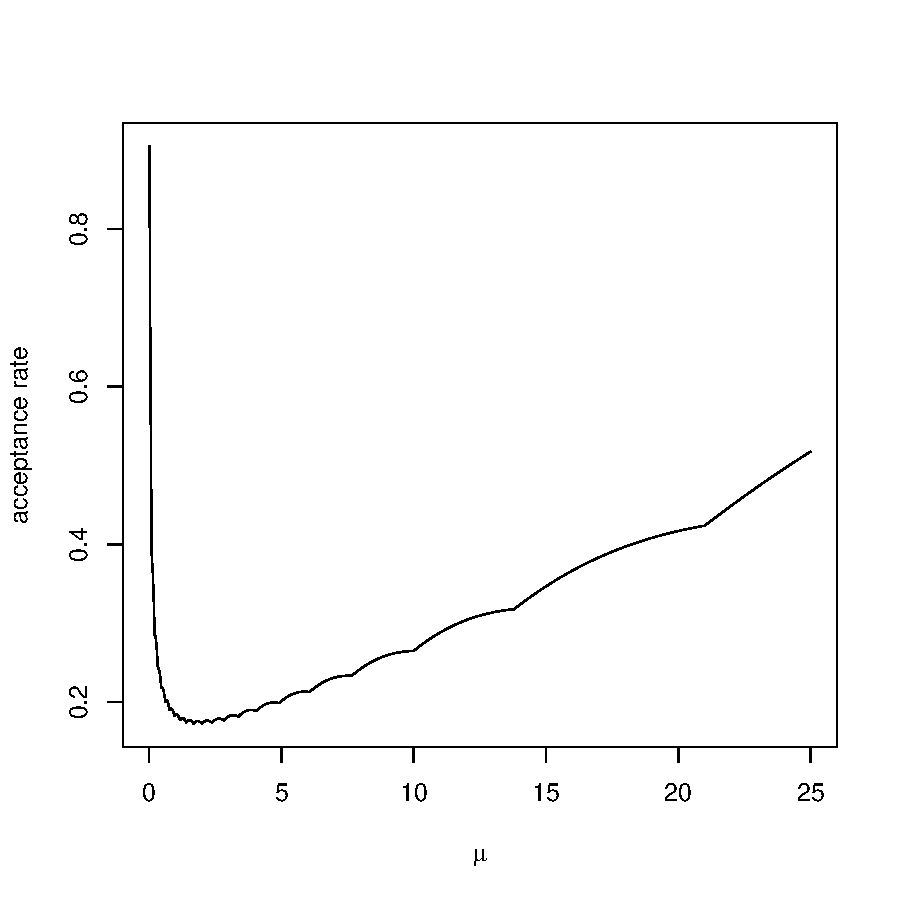
\includegraphics{trunc-fig1}
\end{center}
\caption{Performance of our algorithm for simulating
$k$-truncated negative binomial with $k = 20$,
$\alpha = 2.22$ and $\mu$ plotted.}
\label{fig:fig1}
\end{figure}

The performance is not great, but it will have to do until we find
a better algorithm.

\subsection{Poisson}

We now work out the analogous algorithm for the Poisson distribution.

\subsubsection{Algorithm}

It is clear that taking limits as $\alpha \to \infty$
that the analogous algorithm for Poisson variates is as follows.
The target distribution is $k$-truncated Poisson with untruncated
mean $\mu$.  The proposal is $Y + m$, where $Y$ is untruncated Poisson
with mean $\mu$.

Then the ratio of target PMF to proposal PMF is proportional to
(dropping terms that do not contain $x$)
$$
   r(x)
   =
   \frac { (x - m) !} {x !} \cdot I(x > k)
$$
This is a decreasing function of $x$.
So the acceptance probability can be taken to be
$$
   a(x)
   =
   \frac{r(x)}{r(k + 1)}
   =
   \frac {(k + 1) !} { (k + 1 - m) !}
   \cdot
   \frac { (x - m) !} {x !}
   \cdot
   I(x > k)
$$

\subsubsection{Performance}

To understand the performance of this algorithm, hence to understand how
to chose $m$, we need to calculate the acceptance rate
\begin{align*}
   \rho(m)
   & =
   E^* \{ a(Y + m) \}
   \\
   & =
   \sum_{y = 0}^\infty a(y + m) \frac{\mu^y}{y !} e^{- \mu}
   \\
   & =
   \sum_{y = 0}^\infty
   \frac {(k + 1) !} { (k + 1 - m) !}
   \cdot
   \frac { (y + m - m) !} {(y + m) !}
   \cdot
   I(y + m > k)
   \cdot
   \frac{\mu^y}{y !} e^{- \mu}
   \\
   & =
   \frac {(k + 1) !} { (k + 1 - m) !}
   \sum_{y = k + 1 - m}^\infty
   \frac{\mu^y} {(y + m) !} e^{- \mu}
   \\
   & =
   \frac {(k + 1) !} { (k + 1 - m) !}
   \cdot
   \mu^{- m}
   \sum_{x = k + 1}^\infty
   \frac{\mu^x} {x !} e^{- \mu}
   \\
   & =
   \frac {(k + 1) !} { (k + 1 - m) !}
   \cdot
   \mu^{- m}
   \cdot
   \Prsub{\infty, \mu}\{ Y > k \}
\end{align*}

Everything is fixed in our formula for acceptance rate except $m$,
which we many choose to be any integer $0 \le m \le k + 1$.  Consider
$$
   \frac{\rho(m + 1)}{\rho(m)}
   =
   \frac{(k + 1 - m)}{\mu}.
$$
This is greater than one (so it pays to increase $m$) when
$$
   k + 1 - m < \mu.
$$
Hence we set
$$
   m = \lceil k + 1 - \mu \rceil
$$
or zero, whichever is greater.

\subsubsection{Checks}

There are a lot of thing to check about our analysis.
First we need to check that we actually have a valid rejection sampling
algorithm.
\begin{Schunk}
\begin{Sinput}
> mu <- 2.22
> k <- 20
> m <- max(ceiling(k + 1 - mu), 0)
> m
\end{Sinput}
\begin{Soutput}
[1] 19
\end{Soutput}
\begin{Sinput}
> nsim <- 1e+06
> y <- rpois(nsim, lambda = mu)
> xprop <- y + m
> aprop <- exp(lfactorial(y) - lfactorial(xprop) + lfactorial(k + 
+     1) - lfactorial(k + 1 - m)) * as.numeric(xprop > 
+     k)
> max(aprop)
\end{Sinput}
\begin{Soutput}
[1] 1
\end{Soutput}
\begin{Sinput}
> x <- xprop[runif(nsim) < aprop]
> n <- length(x)
> fred <- tabulate(x)
> xfred <- seq(along = fred)
> pfred <- dpois(xfred, lambda = mu)
> pfred[xfred <= k] <- 0
> pfred <- pfred/sum(pfred)
> mfred <- max(xfred[n * pfred > 5])
> o <- fred
> o[mfred] <- sum(o[seq(mfred, length(fred))])
> o <- o[seq(k + 1, mfred)]
> e <- n * pfred
> e[mfred] <- sum(e[seq(mfred, length(fred))])
> e <- e[seq(k + 1, mfred)]
> chisqstat <- sum((o - e)^2/e)
> pchisq(chisqstat, lower.tail = FALSE, df = length(o))
\end{Sinput}
\begin{Soutput}
[1] 0.09836281
\end{Soutput}
\end{Schunk}
Seems to be o.~k.  (This number changes every time \verb@Sweave@ is run
due to randomness in the simulation.)

Next we check that our performance formula is correct.
\begin{Schunk}
\begin{Sinput}
> length(x)/nsim
\end{Sinput}
\begin{Soutput}
[1] 0.297273
\end{Soutput}
\begin{Sinput}
> rho <- function(m, mu) {
+     exp(lfactorial(k + 1) - lfactorial(k + 1 - m) - m * 
+         log(mu) + ppois(k, lambda = mu, lower.tail = FALSE, 
+         log.p = TRUE))
+ }
> rho(m, mu)
\end{Sinput}
\begin{Soutput}
[1] 0.2975126
\end{Soutput}
\end{Schunk}

Finally, we check the performance of the algorithm over the range of
mean values for which it may have trouble, from zero to a little more
than $k$.
\begin{Schunk}
\begin{Sinput}
> mu <- seq(0.01, k + 5, 0.01)
> m <- pmax(ceiling(k + 1 - mu), 0)
> r <- rho(m, mu)
\end{Sinput}
\end{Schunk}
Figure~\ref{fig:fig2} (page~\pageref{fig:fig2})
shows the performance as a function of $\mu$.
\begin{figure}
\begin{center}
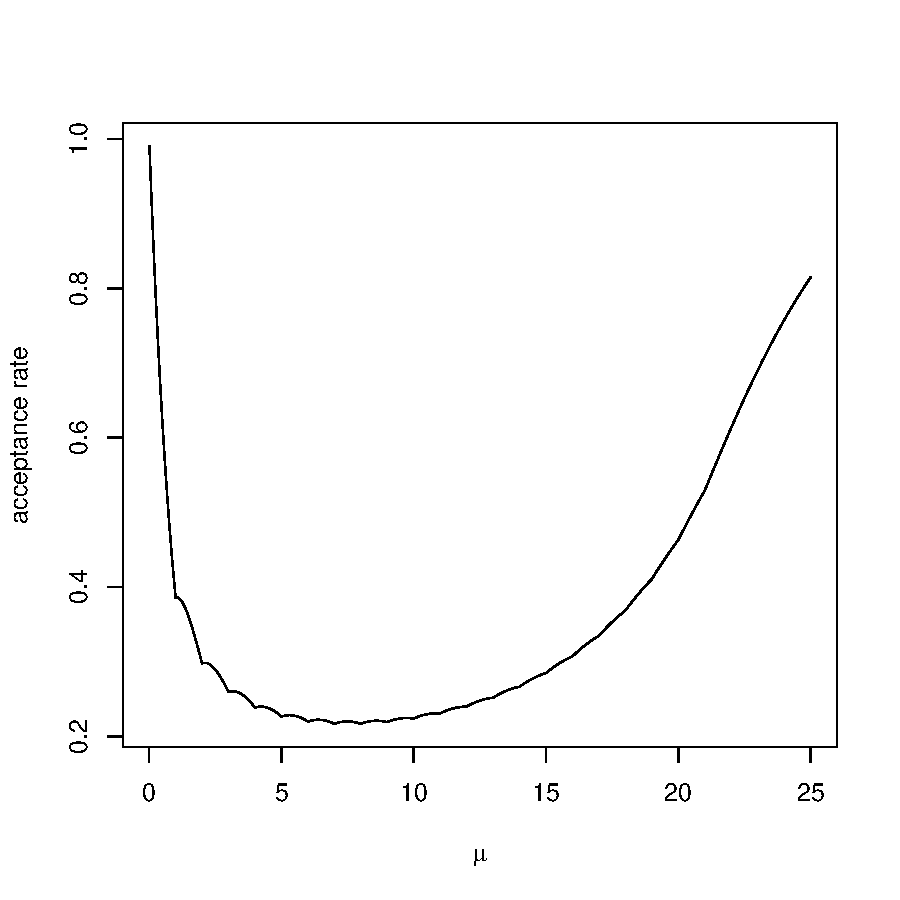
\includegraphics{trunc-fig2}
\end{center}
\caption{Performance of our algorithm for simulating
$k$-truncated poisson with $k = 20$ and $\mu$ plotted.}
\label{fig:fig2}
\end{figure}

\begin{Schunk}
\begin{Sinput}
> kseq <- c(0, 1, 2, 20, 100)
> mseq <- double(length(kseq))
> for (i in seq(along = kseq)) {
+     k <- kseq[i]
+     mu <- seq(0.01, k + 5, 0.01)
+     m <- pmax(ceiling(k + 1 - mu), 0)
+     r <- rho(m, mu)
+     mseq[i] <- min(r)
+ }
\end{Sinput}
\end{Schunk}

The performance of this algorithm seems to be fine for small $k$.
However the worst case acceptance rate, which occurs
for $\mu$ between $k / 4$ and $k / 2$,
does seem to go to zero as $k$ goes to infinity.
For a zero-truncated Poisson distribution the worst case acceptance
rate is 63.2\%.
For a two-truncated Poisson distribution the worst case acceptance
rate is 48.2\%.
For a twenty-truncated Poisson distribution the worst case acceptance
rate is 21.7\%.
For a one-hundred-truncated Poisson distribution the worst case acceptance
rate is 10.2\%.

\end{document}

\begin{center} \LARGE REVISED DOWN TO HERE \end{center}

